\documentclass[11pt,a4paper]{book}
\usepackage[tmargin=2cm, bmargin=3cm, lmargin=2cm, rmargin=2cm]{geometry}
\usepackage[english]{babel}
\usepackage{fancyhdr}
\usepackage{titling}
% Optional
\usepackage{listings}
\usepackage{xcolor}
\usepackage{lipsum}
\usepackage{textcomp}
\usepackage{subfiles}
\usepackage[hidelinks]{hyperref}
\usepackage{pdfpages}
\usepackage{csquotes}

%Bibliography setup
\usepackage[
backend=bibtex,
style=alphabetic,
sorting=ynt
]{biblatex}

\addbibresource{codeprint.bib}

% Titleplage
\title{Code Printing for EOPL}
\date{\today}
%TODO: add your name here if you helped.
\author{Dieter Castel, \\ Karel Domin, \\ Dennis Frett, \\ Jonas Devlieghere,}


\usepackage{listings}
\usepackage{color}
\definecolor{mygreen}{rgb}{0,0.6,0}
\definecolor{mygray}{rgb}{0.5,0.5,0.5}
\definecolor{mymauve}{rgb}{0.58,0,0.82}
% Scheme highlighting

\definecolor{mauve}{rgb}{0.58,0,0.82}

\lstset{%
  backgroundcolor=\color{white},
  basicstyle=\footnotesize,
  breakatwhitespace=false,
  breaklines=true,
  captionpos=b,
  deletekeywords={...},
  escapeinside={\%*}{*)},
  frame=single,
  keepspaces=true,
  language=Scheme,
  morekeywords={cases},
  numbers=left,
  numberstyle=\small\ttfamily\color{gray},
  rulecolor=\color{black},
  stringstyle=\color{mauve},
  showspaces=false,
  showstringspaces=false,
  showtabs=false,
  stepnumber=1,
  tabsize=2,
  title=\lstname
}

%TODO: if someone really wants to define styles for all our lovely languages.
% \lstdefinestyle{}{
% }


%README:
%Refer to the code that is in this repository
%Only include those lines of the code that are vital to understanding it
%Try to reduce the amount of code as much as you can.
%If you need to change 3 lines in a syntax file include those lines
%only with some added context (like in which function you are editing it).
%If you want to add extra comment add it in the actual language racket file

\begin{document}
\frontmatter
\maketitle
\tableofcontents

\mainmatter
\setcounter{chapter}{2}
\chapter{Expressions}

\section{LET}
\subfile{subfiles/LET.tex}

\section{LETREC}
\subfile{subfiles/LETREC.tex}

\chapter{State}

\section{EXPLICIT-REFS}
\subfile{subfiles/EXPLICIT-REFS.tex}

\section{IMPLICIT-REFS}
\subfile{subfiles/IMPLICIT-REFS.tex}

\chapter{Continuation-Passing Style}

\section{THREADS}
\subfile{subfiles/THREADS.tex}

\setcounter{chapter}{6}
\chapter{Types}

\section{CHECKED)}
\subfile{subfiles/CHECKED.tex}

\chapter{Modules}

\section{SIMPLEMODULES}
\subfile{subfiles/SIMPLEMODULES.tex}

\chapter{Objects \& Classes}

\section{CLASSES}
\subfile{subfiles/CLASSES.tex}

\chapter{Exercises}
\subfile{subfiles/exercises.tex}
\section{Contour diagrams}
%Contributed by Karel Domin
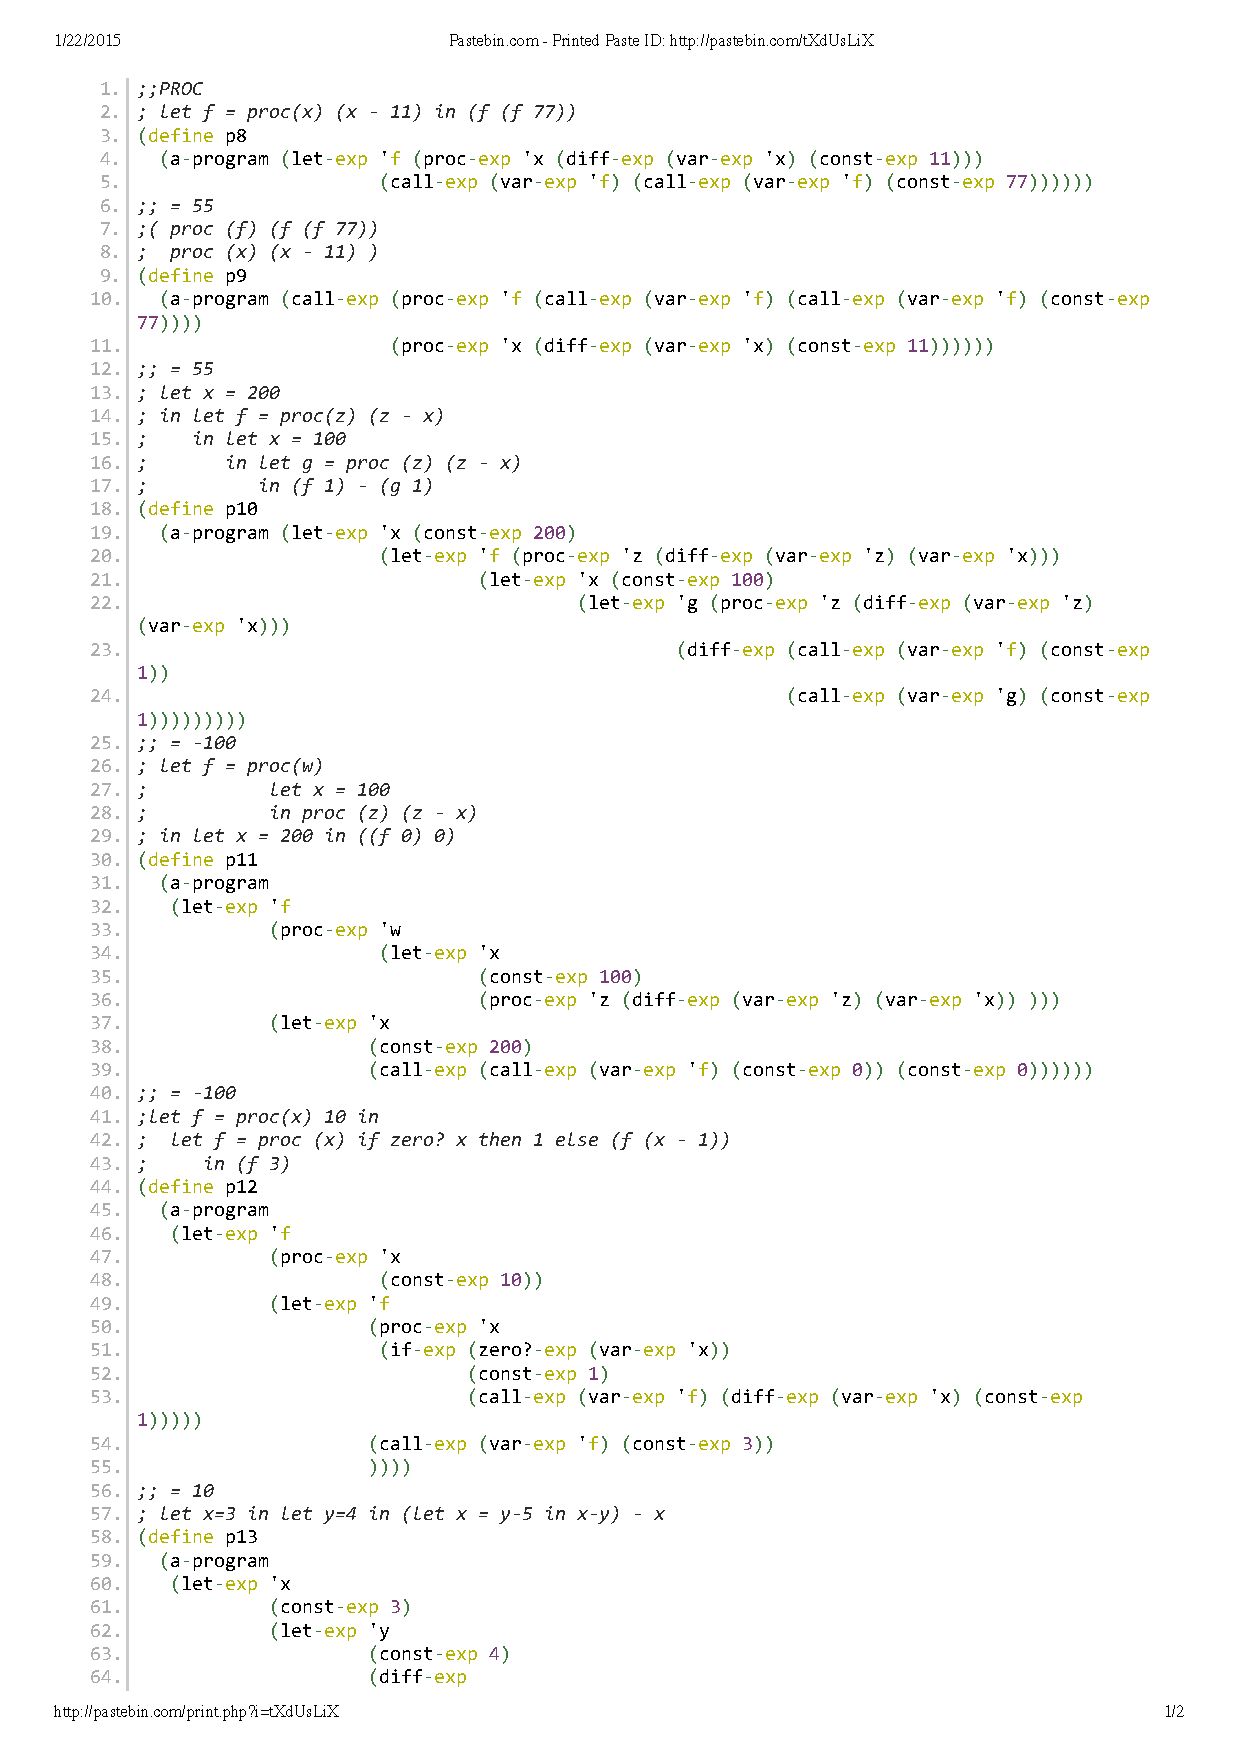
\includepdf[pages={1,3-},landscape=false,pagecommand=\thispagestyle{plain}]{subfiles/Exc1.pdf}

\backmatter
\appendix

\nocite{*}
\printbibliography
\end{document}
